\subsection{Inviscid Flux Schemes}

The default inviscid flux used in the {\it flowPsi} is Torro's HLLC
scheme \cite{Torro.1994}.  However, a low dissipation flux is also
available when may be enabled by setting the {\tt inviscidFlux} to
either 'kec' or 'ssf'.  The 'ssf' scheme will revert to a $4^{th}$
order accurate skew symmetric scheme on Cartesian meshes.

\subsection{Preconditioned HLLC flux option}

The robust Chorin-Turkel preconditioning is implemented to facilitate
efficient and accurate solution for low speed flows.  This is
particularly useful for RANS computations.  Preconditioning provides
two benefits for approximate Riemann solver codes.  First,
preconditioning rescales the acoustic wave speeds to be comparable in
magnitude to the convective waves.  This allows for improved iterative
convergence to the steady state solution.  Second, preconditioning
reduces the dissipation of standard flux schemes such as HLLC.  For
flows below about Mach 0.2, the dissipation of the scheme can make
accurate solution difficult or impossible.

\subsubsection{Background on preconditioning}

The basic idea behind preconditioning is the provision of modified
time derivative which rescales the the acoustic wave speeds without
changing the convective wave speeds.  The time derivative for preconditioning is modified in the following way:

\begin{equation}
  M P^{-1} \frac{\partial q}{\partial t} = div(F(q)) + div(F_v(q))
\end{equation}
where $q=[T, \mathbf{u}, p_g]^T$ is the primitive vector, $M$ is the conservative transformation matrix and $P^{-1}$ is the inverse of the preconditioning matrix.  The conservative transformation matrix is given by
\begin{equation}
\frac{\partial Q}{\partial q} = M=\left[
{\begin{array}{cccccc}
-\frac{\rho}{T}   & 0    & 0 & 0 & \frac{\rho}{\tilde{R} T}  \\
-\frac{\rho u}{T} & \rho & 0 & 0 & \frac{\rho u}{\tilde{R} T} \\
-\frac{\rho v}{T} & 0 & \rho & 0 & \frac{\rho v}{\tilde{R} T} \\
-\frac{\rho w}{T} & 0& 0 & \rho  & \frac{\rho w}{\tilde{R} T} \\
f_T & \rho u & \rho v & \rho w & f_p\\
\end{array}}
\right],
\end{equation}
where $f_T$ and $f_p$ are the derivatives of $\rho e_0$ with respect to pressure and temperature which is given as
\begin{equation}
f_T= -\frac{\rho h_0}{T} + \frac{\gamma}{\gamma-1} \rho \tilde{R},
\end{equation}
and
\begin{equation}
f_p= \frac{h_0}{\tilde{R} T} - 1 
\end{equation}

The preconditioning matrix is given by
\begin{equation}
{\bf P} = \left[
{\begin{array}{ccccc}
1 & 0 & 0 & 0 & -\frac{(1-\eta_p)(\gamma-1) T}{a^2 \rho}  \\
0 & 1 & 0 & 0 & 0 \\
0 & 0 & 1 & 0 & 0 \\
0 & 0 & 0 & 1 & 0 \\
0 & 0 & 0 & 0 & \eta_p  \\
\end{array}}
\right]
\end{equation}
The inverse of ${\bf P}$ can be found as 
\begin{equation}
{\bf P}^{-1} = \left[
{\begin{array}{ccccc}
1 & 0 & 0 & 0 & -\frac{(1-1/\eta_p)(\gamma-1) T}{a^2 \rho}  \\
0 & 1 & 0 & 0 & 0 \\
0 & 0 & 1 & 0 & 0 \\
0 & 0 & 0 & 1 & 0 \\
0 & 0 & 0 & 0 & 1/\eta_p  \\
\end{array}}
\right],
\end{equation}
where $\eta_p$ is the preconditioning parameter which is given by
\begin{equation}
  \eta_p = M_r^2/(1-M_r^2)
\end{equation}
where $M_r$ is a local Mach number which is bounded such that $M_r^2 \le \frac{1}{2}$.  In addition, to prevent instability in the case caused by Mach number approaching zero, a lower bound on $M_r$ is provided based on an estimated free stream mach number provided by the user.


The eigenvalues for this modified system of equations are given by
\begin{equation}
\Lambda=[u_n,u_n,u_n, \frac{u_n(1+\eta_p)-\sigma}{2},\frac{u_n(1+\eta_p)+\sigma}{2}].
\end{equation}
where $\sigma=\sqrt{u_n^2(1-\eta_p)^2+4\eta_pa^2}$.


The change in wave speeds by the preconditioning matrix changes the
eigenvectors and eigenvalues associated with the approximate Riemann
solver.  In the case of the HLLC flux, it is sufficient to modify the
eigenvalues used in the construction of the HLLC flux. For a Roe based
scheme the new eigenvectors are used to construct a preconditioned Roe
matrix.  We use the modified HLLC scheme on the RHS of the equations,
but use the preconditioned Roe matrix as an approximate linearization.

\subsubsection{Skew Symmetric low dissipation flux schemes}


Our goal is to develop a low dissipation numerical scheme for
unstructured grids by forming a hybrid of a low dissipation skew
symmetric flux designed for Cartesian meshes with traditional upwinded
unstructured methods such that we recover the Cartesian mesh algorithm
for regular meshes and also provide a low dissipation characteristic
on irregular meshes.  The Cartesian formulation in which this is based on 
are $2^{nd}$ and $4^{th}$ order fluxes from the skew-symmetric family
of flux functions.  For this discussion, consider the $2^{nd}$ order
skew symmetric flux that is evaluated at cell faces as a function of
averaged variables by the relation
\begin{equation}
F_{avg}(l,r) = \rho(p_{avg},T_{avg}) \left(\vec{u}_{avg}\cdot\vec{n}\right)
\label{eq:cflux}
\begin{bmatrix}
  1\\
\vec{u}_{avg}\\
e(p_{avg},T_{avg}) + k_{avg}\\
\end{bmatrix} +
\begin{bmatrix}
0\\
p_{avg} \vec{n} \\
p_{avg} \left(\vec{u}_{avg}\cdot \vec{n}\right)\\
\end{bmatrix}
\end{equation}
where the density, $\rho(p,T)$, and internal energy, $e(p,T)$, are
provided by the equation-of-state, $\vec{n}$ is the face normal
vector, and the averaged variables $p_{avg}$, $T_{avg}$,
$\vec{u}_{avg}$, and $k_{avg}$ are provided by the following averaging
relations:
\begin{equation}
\begin{aligned}
p_{avg} &= \frac{1}{2}\left(p_l + p_r\right)\\
T_{avg} &= \frac{1}{2}\left(T_l + T_r\right)\\
\vec{u}_{avg} & = \frac{1}{2}\left(\vec{u}_l + \vec{u}_r\right)\\
k_{avg} &= \vec{u}_{avg}\cdot\vec{u}_{avg}-\frac{1}{4} \left( \vec{u}_l\cdot\vec{u}_l + \vec{u}_r\cdot\vec{u}_r\right)\\
\label{eq:averaging}
\end{aligned}
\end{equation}

For an ideal gas, the equations-of-state provide the following functions:
\begin{equation}
\begin{aligned}
\rho(p,T) &= \frac{p}{\tilde{R} T},\\
e(p,T) &= \frac{\tilde{R}}{\gamma-1} T.\\
\end{aligned}
\end{equation}

The above formulation reproduces the compressible kinetic energy
consistent (KEC) form of Subbareddy {\it et al.}\cite{Subbareddy.2009}
due to the definition of average fluid kinetic energy, $k_{avg}$.
However, this scheme differs from the Subbareddy flux form in that
averages of temperature and pressure are formed and then density and
internal energy are derived from the equation-of-state (EoS), whereas
the original KEC flux formed independent averages for these variables.
Other options for averaging, including density and internal energy
averaging, were also evaluated and it was found that the above
averaging process generally produced errors that are lower by a factor
of up to two.

The second order skew-symmetric flux of eq. (\ref{eq:cflux}) can
be used as a basis to construct a $4^{th}$ order scheme following the
construction of Pirozzoli\cite{Pirozzoli.2010,Pirozzoli.2011} and
given here as the form:
\begin{equation}
F_{SSF} = (1+2\beta)F_{avg}(l,r) - \beta\left(F_{avg}(ll,r)+F_{avg}(r,rr)\right),
\label{eq:fourth}
\end{equation}
where $\beta = \frac{1}{6}$ and $ll$ denotes the value of the cell
left-of-left and $rr$ denotes the value of the cell right-of-right.
This $4^{th}$ order skew-symmetric flux (obtained when
$\beta=\frac{1}{6}$) will be denoted as the SSF scheme.  When $\beta =
0$ this flux reduces to the KEC scheme of Subbareddy {\it et al.}.
This flux will provide the central flux scheme in our hybridized low
dissipation scheme.

\subsubsection{Unstructured Mesh Hybridization}

For unstructured solvers we would like to modify the SSF scheme in
such a way that it becomes identical to the $4^{th}$ order scheme on
Cartesian meshes but gracefully degrades to a low dissipation second
order scheme on unstructured meshes.  The flux written in equation
(\ref{eq:fourth}) is not directly applicable to unstructured meshes
because of the direct reference to left-of-left and right-of-right
cells that have no clear definition in an irregular mesh structure.
The general problem is illustrated in Figure \ref{fig:stencil}
where $\vec{x}_l$ and $\vec{x}_r$ denote the cell centroids of the
given polyhedral mesh, $\vec{x}_f$ is the face centroid of a given
polygonal face, while $\vec{x}_c$ is the midpoint location between
the cell faces where the centered flux is defined.  Here
$\vec{x}_{ll}$ and $\vec{x}_{rr}$ are the nominal locations of a
Cartesian mesh overlayed onto this unstructured mesh.  In general no
cells are centered at these locations, but for a Cartesian mesh these
points will correspond to the expected cell centers.  The construction
of an unstructured scheme requires the resolution of two issues: how
to correct for the fact that the flux interpolation center ($X_c$)
does not correspond to the face centroid ($X_f$) and how to obtain
values for the left-of-left and right-of-right values in an
unstructured context.

\begin{figure}[h]
\begin{center}
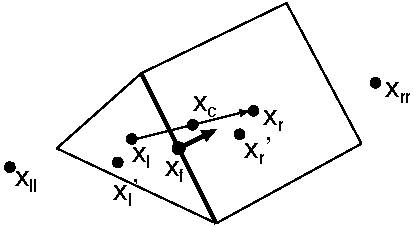
\includegraphics[width=0.5\textwidth]{flux_correct}
\caption{Geometry of flux stencil formation}
\label{fig:stencil}
\end{center}
\end{figure}


We can utilize the cell gradients computed on the left and right side
to devise a correction for the offset between $\vec{x}_f$ and
$\vec{x}_c$.  Note that the without this correction the scheme given
in Eq. (\ref{eq:fourth}) will degrade to first order on unstructured
grids unless mesh refinement is sufficiently smooth
(e.g. $|\vec{x}_f-\vec{x}_c| = O(h^2)$). A correction that will
restore second order accuracy for non-smooth refinements is
accomplished by using the cell centered gradients at the left and
right cells to shift the stencil such that it is centered on the face
center.  For a given interpolated value $\phi$, the states
interpolated to this new stencil are given by the correction
\begin{equation}
\begin{aligned}
{\phi_{l}}^{'} &= \phi_l + \nabla \phi_l \cdot (\vec{x}_f-\vec{x}_c)\\
{\phi_{r}}^{'} &= \phi_r + \nabla \phi_r \cdot (\vec{x}_f-\vec{x}_c),\\
\end{aligned}
\end{equation}
which provides a second order correction provided that $\nabla \phi$
is computed to at least first order accuracy.

To recover a $4^{th}$ order accurate scheme on Cartesian meshes we
need to establish a reconstruction for the left-of-left and
right-of-right stencil locations that will correspond to the actual
values at these cell locations on a Cartesian mesh, but are only
functions of the available left and right values and gradients.  To do
this we start with the assumption that gradients will be computed at
the cells using a least squares reconstruction.  For this
reconstruction on a Cartesian mesh, it can be show that the following
relationships will identically hold:
\begin{equation}
\begin{aligned}
\nabla \phi_l \cdot (\vec{x}_r-\vec{x}_l) = &\frac{\phi_{r}-\phi_{ll}}{2}\\
\nabla \phi_r \cdot (\vec{x}_r-\vec{x}_l) = &\frac{\phi_{rr}-\phi_{l}}{2}\\
\end{aligned}
\end{equation}

Using these relations, we can then compute an effective left-of-left
and right-of-right state using the cell values and their gradients.
These are defined as follows:
\begin{equation}
\begin{aligned}
{\phi_{ll}}^{'} &= {\phi_r}^{'} - 2 \nabla \phi_l \cdot (\vec{x}_r-\vec{x}_l) \\
{\phi_{rr}}^{'} &= {\phi_l}^{'} + 2 \nabla \phi_r \cdot (\vec{x}_r-\vec{x}_l) \\
\end{aligned}
\end{equation}

The approach produces exactly the $4^{th}$ order flux on Cartesian
grids and also provides a reasonable correction for general meshes.
This approach has the advantage of only requiring the cell centered
least squares gradient which will be required for the upwind flux as
was observed in a similar formulation presented by Darwish and
Moukalled\cite{Darwish.2003}.  Note, this implementation was arrived at
after evaluating many subtle variations on the themes presented here.
For example, a centered face interpolation using cubic polynomials is
evaluated to replace the face averaged values for the skew-symmetric
flux but did not produce $4^{th}$ order convergence on Cartesian
meshes due to the presence of aliased second order modes.  Similarly,
centered linear reconstructions at the face were evaluated to correct
for location of the face center, but the resulting scheme is less
stable and required more blended upwinding than the one presented
here.

\subsubsection{Hybrid Flux Scheme}

In practice the skew symmetric fluxes (equation (\ref{eq:fourth}))
fail for shocked flows and therefore need to be hybridized with standard
upwind fluxes to enable simulation of high speed flows.  In addition,
unstructured stencils can depart significantly from skew-symmetry and
thus will require some stabilizing dissipation which is provided by
blending to the upwind flux. This blending is achieved by using a
simple weighted average of central flux and upwind flux schemes such
that our final inviscid flux can be written as
\begin{equation}
F_i = (1-\alpha_{diss})F_{SSF} + \alpha_{diss} F_{upwind}.
\end{equation}
For this study we utilize the robust HLLC scheme\cite{Torro.1994} for
the upwind flux.  Since we are also using the upwind scheme to
stabilize corrections on unstructured meshes we modify the 
upwind scheme to provide low dissipation in low Mach number regions by
employing the simple scaling scheme proposed by Thornber {\it et
  al.}\cite{Thornber.2008} whereby the left and right velocity states
are modified according to the local face Mach number, $M_{f}$,
according to the relations:
\begin{equation}
\begin{aligned}
\vec{u}_{l,th} &= \frac{\vec{u}_l + \vec{u}_r}{2} + \min(M_{f},1) \frac{\vec{u}_l-\vec{u}_r}{2}\\
\vec{u}_{r,th} &= \frac{\vec{u}_l + \vec{u}_r}{2} + \min(M_{f},1) \frac{\vec{u}_r-\vec{u}_l}{2}\\
\end{aligned}
\end{equation}

Blending upwind fluxes will be motivated by three concerns: 1)
geometric concerns where upwinding is used to stabilize the central
flux schemes when skew-symmetry is lost, and 2) to provide a proper
amount of added dissipation in regions with dissipative structures
such as shocks and expansions, and 3) to provide a Monotone Implicit
LES model (MILES) approach to subgrid filtering by employing a small
amount of upwinding dissipation as an implicit subgrid model.
Therefore $\alpha_{diss}$ will be computed based on mesh geometry
($\alpha_{geom}$) and compressibility based ($\alpha_{comp}$), and
subgrid modeling based ($\alpha_{miles}$) considerations.  Ultimiately
$\alpha_{diss}$ will be determined by the maximum of these three
factors.  Since blending to upwinding generally introduces dissipation
to the scheme, we would like to keep the non-physics based
$\alpha_{geom}$ as small as possible.  We use a heuristic approach to
add dissipation based on angles formed by the face reconstruction
where each face blends to an upwind scheme independently.
Specifically we are concerned with two potentially problematic angles:
1) the angle between the face normal and the vector joining the cell
center should be as close to zero as possible, and 2) the angle of a
line that is tangent to a sphere centered on the skew-symmetric flux
center ($X_c$) with a radius containing the face centroid, $r_f =
|X_f-X_c|$ as illustrated in figure \ref{fig:stencilangle}.  The
geometric upwinding is computed based on the maximum of these two
angles, denoted as $\theta_{max}$.  Then the geometric based upwinding
is computed using the relation
\begin{equation}
\alpha_{geom} = \chi^2 + \frac{\eta_2}{\eta_1}*(\chi^3-2\chi^2+\chi); \chi
= \min\lbrace\eta_1(1-\cos~\theta_{max}),1\rbrace
\end{equation}
where $\eta_1$ selects the angle at which full upwinding will occur,
and $\eta_2$ controls how fast upwinding is added for small departures
from ideal mesh quality.  For the test cases studied it was found that
accurate and robust results were obtained with, $\eta_1=2$, which
provides full upwinding when $\theta_{max} = 60\deg$, while $\eta_2=1$
ensures stability on good quality meshes where small corrections are
applied keeping $\alpha_{geom} \sim 1-cos~\theta_{max}$ for small
angles.  In general, $\eta_1$ and $\eta_2$ are user adjustable
parameters, but the settings described here are effective for a wide
range of mesh configurations and appear to provide a reasonable
compromise between robustness and low dissipation.

\begin{figure}[h]
\begin{center}
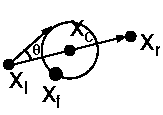
\includegraphics[width=0.5\textwidth]{geom_test}
\caption{Geometry of flux stencil formation}
\label{fig:stencilangle}
\end{center}
\end{figure}

Since the central flux scheme cannot properly resolve shocks, a method
must be used to identify regions of the flow that have shocks where it
is necessary to switch to an upwind scheme.  One of the more popular
shock detectors used for this purpose is the method originally
implemented by Ducros {\it et al.}\cite{Ducros.2000} which detects
shocks by comparing the magnitude of the divergence of velocity with
the vorticity.  Regions that are vorticity dominant (such as LES
regions) switch to the low dissipation flux.  However, this switch
often becomes active in regions where an upwind scheme is not
necessary.  In addition, refining a region of smooth flow will not
allow the code to switch to a lower dissipation flux.  Ideally a
switch should reduce the area where the upwind scheme is utilized with
mesh refinement, and so a switch that considers local mesh resolution
is desired.  This switch should be based on the magnitude of
divergence of the velocity field which gives a measure of the
rate of compression in the flow, a mesh length scale, and some measure of
the fluid response to compression, such as sound speed.  Using these
measures and dimensional analysis we arrive at the following
\begin{equation}
\alpha_{comp} = \left[\min\left(\eta_{comp}\frac{\left| \nabla \cdot
        \vec{u} \right| \delta x_{ref}}{a },1\right)\right]^2
\label{eq:alphacomp}
\end{equation}
where $a$ is the local sound speed, and $\delta x_{ref}$ is the cell
reference length defined as the diameter of the smallest sphere that
encloses all cell face centers.  The variable $\eta_{comp}$ is a user
defined sensitivity parameter.  The non-dimensional term is squared so
that the transition to the central scheme will correspond with mesh
refinement at a rate of $O(h^2)$ in smooth flow regions.  For the
studies that involve shocks presented here a value of $\eta_{comp} =
5$ is used.  Note, with this method the value for $\alpha_{comp}$ will
vanish with mesh refinement for any smooth solution, but will always
be active at shocks.  The final value for $\alpha_{diss}$ used by the
flux is defined by the maximum of the left and right values for
$\alpha_{comp}$ and the local face value for $\alpha_{geom}$.
